\section{Modification dans la conception}

Au cours du projet, nous avons réalisé un schéma de conception logicielle, expliquant comment s'organisaient les scripts les uns par rapport aux autres.
Tout au long de l'implémentation, et bien que nous ayons gardé  en tête le schéma initial, certains facteurs ont fait diverger la conception logicielle réelle de celle prévue.
Parmi ces facteurs, on compte notamment Middle VR et Unity.

\subsection{Middle VR : des imprévus au programme}

Middle VR est une couche logicielle d'abstraction permettant de développer une solution logicielle et de l'utiliser telle quelle avec n'importe quel périphérique de réalité virtuelle.
Il permet, sans modifier la solution, de l'utiliser indifféremment avec un casque de réalité virtuelle ou la faire fonctionner en salle immersive.
Néanmoins Middle VR pose quelques problèmes lorsque l'on veut l'utiliser avec un couple clavier/souris - qui n'est pas un adapté à la réalité virtuelle.
Par exemple, les valeurs de position/rotation de certains objets sont gérés par Middle VR (par exemple le VR Center Node, Head Node, ...). \\
De plus, Middle VR fonctionne en mode tracker : il capte la position des périphériques pour positionner l'utilisateur dans la scène.
Or, si on est physiquement limité (dans une salle immersive par exemple) avec des périphériques de réalité virtuelle, cela n'est pas le cas avec une souris par exemple.
En effet, rien n'empêche l'utilisateur de soulever la souris pour la reculer et donc avancer en continu, et ceci peut poser certains problèmes dans un logiciel de réalité virtuelle.  

\begin{figure}[h]
	\centering
		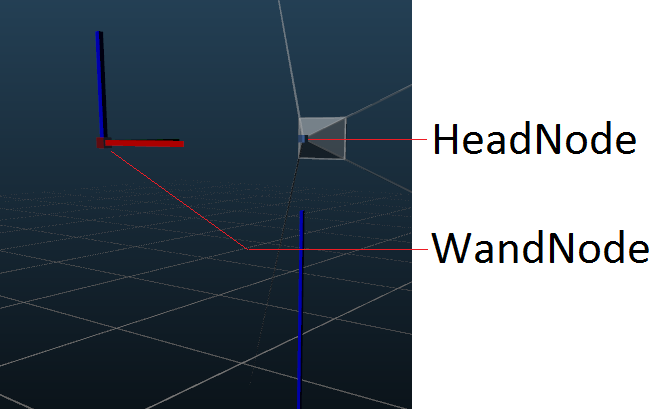
\includegraphics[width=\linewidth]{7-RapportFinal/img/middleVR.PNG}
		\caption{Nodes Middle VR}
		\label{middleVR}
	
\end{figure}

\subsection{Unity : Programmation orientée composants}

Unity fonctionne avec des scripts C\#, attachés en tant que composants sur des objets de la scène (des GameObject).
Pour cela, Unity a son propre compilateur, et son comportement peu parfois être limitant.
Par exemple l'utilisation de pointeurs, bien que fortement déconseillée en C\#, est presque impossible avec Unity. De plus, de par son fonctionnement (orienté composants), l'héritage pose des problèmes sur les scripts qui ont des fonctions update et start.
En effet, start est une fonction lancée - après les constructeurs - au lancement du script, et Update est appelée une fois par frame.
Or, une fonction update ou start peut nécessiter l'éxécution de celle d'un autre script. Pour ces raisons (entre autres), les classes ont du être adaptées.

\subsection{Classes conservées}

Sur le diagramme de classe ci-dessus, la ligne rouge est une démarcation entre les classes qui sont restées presque inchangées dans l'implémentations, et celles qui ne sont pas représentées ou qui ne présentent plus les même caractéristiques. En haut de ladite ligne rouge, sont les classes préservées dans l'implémentation : en effet, la plupart sont abstraites et ne dépendent que des classes standard d'Unity.

\begin{figure}[h]
	\centering
		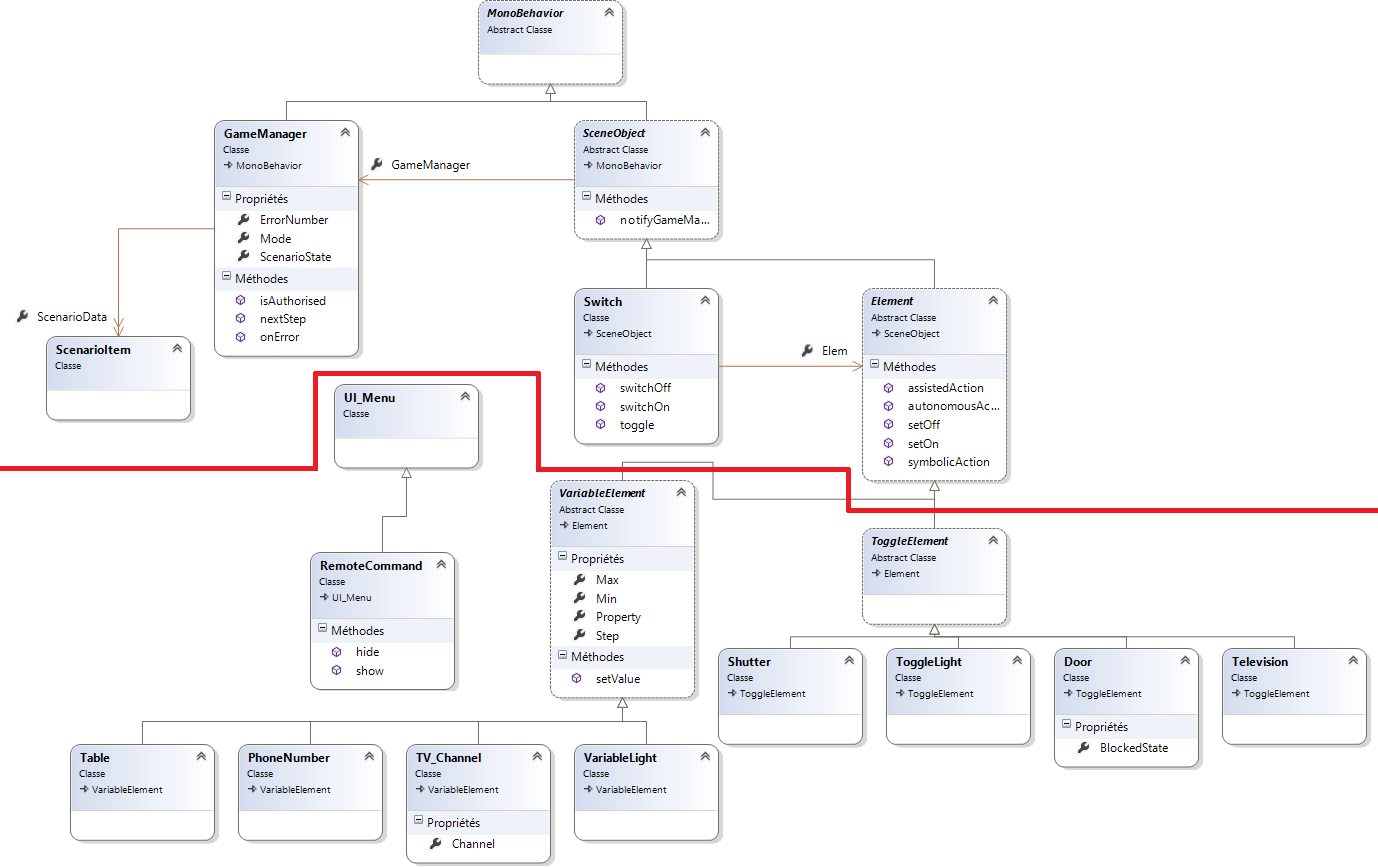
\includegraphics[width=\linewidth]{7-RapportFinal/img/diagClasses_rectif.png}
		\caption{Diagramme de classe initial}
		\label{diagClasses_rectif}
	
\end{figure}

Globalement, même si certaines classes ont disparues ou dont été modifiées, l'architecture générale du projet est respectée. L'ensemble est cohérent avec le schéma initial, même s'il n'est pas rigoureusement identique.






